\chapter{\mypyvy}
\label{chap:mypyvy}

\section{Introduction}

Our experience with \Verdi and \disel has been
  that the most challenging aspect of distributed systems verification
  is discovering inductive invariants.
An inductive invariant is a property of system states that simultaneously
  (1) summarizes all the reachable states of the system,
  (2) is closed under all steps the system can take, and
  (3) ensures the absence of safety violations.
This challenge has led researchers to investigate
  techniques for automatically inferring inductive invariants,
  given a description of a system and its safety property.

This chapter describes \mypyvy
  a tool for automated reasoning
  about symbolic transition systems in first-order logic
  that supports a variety of automated reasoning techniques to analyze systems.
\mypyvy takes an input file
  describing a symbolic transition system
  and performs the analysis requested by the user.
Three of the most interesting analyses include
  inductive invariant checking,
  inductive invariant inference, and
  bounded trace reasoning, including bounded model checking.
In all cases, \mypyvy loads the transition system
  and compiles it together with the user-requested analysis
  to a (sequence of) SMT queries,
  which are dispatched by Z3.

\mypyvy is not just the sum of the analyses currently available;
  it is a platform for doing research in automated verification.
We have ongoing projects that use the \mypyvy foundation
  to build several new invariant inference techniques
  and user interfaces for verification and exploration.
In this context, \mypyvy can be seen as a sort of intermediate language
  that captures the right level of abstraction for implementing
  invariant inference techniques.
Higher level languages, such as \ivy~\cite{Padon-al:PLDI16}
  that want to leverage invariant inference
  can express their queries in \mypyvy and
  use the available inference algorithms.
There is much exciting work to be done here.
This chapter is more modest in scope,
  describing the core of \mypyvy in theory and implementation.

\section{Background on Transition Systems}

\subsection{The robot example informally and pictorially}

\def\xMin{-8}
\def\xMax{8}
\def\yMin{-5}
\def\yMax{11}

\begin{figure}[t]
  \hfil%
  \begin{minipage}{0.45\linewidth}
    \centering
    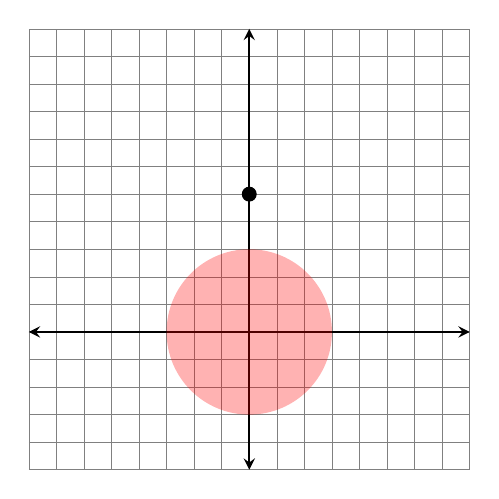
\begin{tikzpicture}[scale=0.35, >=stealth]
      \foreach \i in {\xMin,...,\xMax} {
          \draw [very thin,gray] (\i,\yMin) -- (\i,\yMax);
      }
      \foreach \i in {\yMin,...,\yMax} {
          \draw [very thin,gray] (\xMin,\i) -- (\xMax,\i);
      }
      \draw[<->, thick] (\xMin, 0) -- (\xMax, 0);
      \draw[<->, thick] (0, \yMin) -- (0, \yMax);
      \fill[fill=red, fill opacity=0.3] (0, 0) circle [radius=3];
      \draw[fill=black] (0, 5) circle [radius=0.25];
    \end{tikzpicture}
    \caption{Robot initial configuration.}
    \label{fig:robot-init}
  \end{minipage}%
  \hfil%
  \begin{minipage}{0.45\linewidth}
    \centering
    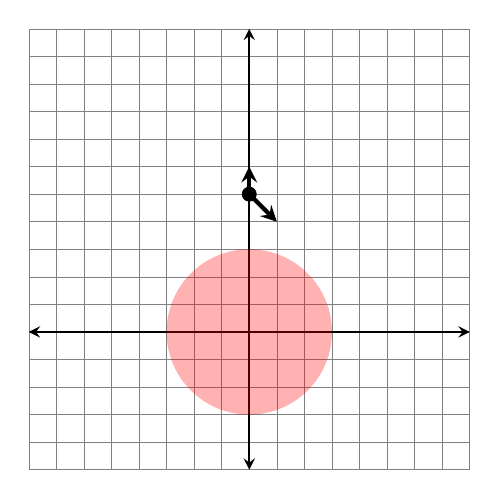
\begin{tikzpicture}[scale=0.35, >=stealth]
      \foreach \i in {\xMin,...,\xMax} {
          \draw [very thin,gray] (\i,\yMin) -- (\i,\yMax);
      }
      \foreach \i in {\yMin,...,\yMax} {
          \draw [very thin,gray] (\xMin,\i) -- (\xMax,\i);
      }
      \draw[<->, thick] (\xMin, 0) -- (\xMax, 0);
      \draw[<->, thick] (0, \yMin) -- (0, \yMax);
      \fill[fill=red, fill opacity=0.3] (0, 0) circle [radius=3];
      \draw[fill=black] (0, 5) circle [radius=0.25];
      \draw[->, line width=1.5pt] (0, 5) -- (0, 6);
      \draw[->, line width=1.5pt] (0, 5) -- (1, 4);
    \end{tikzpicture}
    \caption{Robot's first steps.}
    \label{fig:robot-first-steps}
  \end{minipage}%
  \hfil%
  \hrule
  \vspace{1em}
  \begin{minipage}{1\linewidth}
    \centering
    \begin{minipage}{0.5\linewidth}
      \centering
      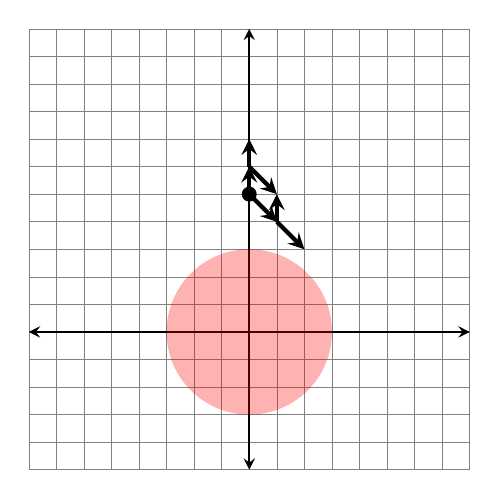
\begin{tikzpicture}[scale=0.35, >=stealth]
        \foreach \i in {\xMin,...,\xMax} {
            \draw [very thin,gray] (\i,\yMin) -- (\i,\yMax);
        }
        \foreach \i in {\yMin,...,\yMax} {
            \draw [very thin,gray] (\xMin,\i) -- (\xMax,\i);
        }
        \draw[<->, thick] (\xMin, 0) -- (\xMax, 0);
        \draw[<->, thick] (0, \yMin) -- (0, \yMax);
        \fill[fill=red, fill opacity=0.3] (0, 0) circle [radius=3];
        \draw[fill=black] (0, 5) circle [radius=0.25];
        \draw[->, line width=1.5pt] (0, 5) -- (0, 6);
        \draw[->, line width=1.5pt] (0, 5) -- (1, 4);
        \draw[->, line width=1.5pt] (0, 6) -- (0, 7);
        \draw[->, line width=1.5pt] (0, 6) -- (1, 5);
        \draw[->, line width=1.5pt] (1, 4) -- (1, 5);
        \draw[->, line width=1.5pt] (1, 4) -- (2, 3);
      \end{tikzpicture}%
    \end{minipage}%
    \begin{minipage}{0.5\linewidth}
      \centering
      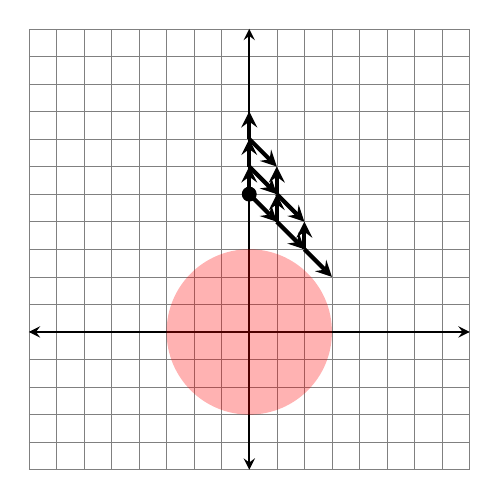
\begin{tikzpicture}[scale=0.35, >=stealth]
        \foreach \i in {\xMin,...,\xMax} {
            \draw [very thin,gray] (\i,\yMin) -- (\i,\yMax);
        }
        \foreach \i in {\yMin,...,\yMax} {
            \draw [very thin,gray] (\xMin,\i) -- (\xMax,\i);
        }
        \draw[<->, thick] (\xMin, 0) -- (\xMax, 0);
        \draw[<->, thick] (0, \yMin) -- (0, \yMax);
        \fill[fill=red, fill opacity=0.3] (0, 0) circle [radius=3];
        \draw[fill=black] (0, 5) circle [radius=0.25];
        \draw[->, line width=1.5pt] (0, 5) -- (0, 6);
        \draw[->, line width=1.5pt] (0, 5) -- (1, 4);
        \draw[->, line width=1.5pt] (0, 6) -- (0, 7);
        \draw[->, line width=1.5pt] (0, 6) -- (1, 5);
        \draw[->, line width=1.5pt] (1, 4) -- (1, 5);
        \draw[->, line width=1.5pt] (1, 4) -- (2, 3);
        \draw[->, line width=1.5pt] (0, 7) -- (0, 8);
        \draw[->, line width=1.5pt] (0, 7) -- (1, 6);
        \draw[->, line width=1.5pt] (1, 5) -- (1, 6);
        \draw[->, line width=1.5pt] (1, 5) -- (2, 4);
        \draw[->, line width=1.5pt] (2, 3) -- (2, 4);
        \draw[->, line width=1.5pt] (2, 3) -- (3, 2);
      \end{tikzpicture}
    \end{minipage}%
    \caption{Robot's second and third steps.}
    \label{fig:robot-23-steps}
  \end{minipage}
\end{figure}

Imagine a robot in a 2-dimensional world.
The robot starts at position $(0, 5)$,
  and can take steps to integer grid points either
 due north or diagonally southeast of its current position.
The world has a circular hole of radius 3 centered at the origin.
Can the robot ever fall in the hole?\footnote{Thanks to Jon Howell for this example.}

The initial situation is depicted in \cref{fig:robot-init}.
The smaller black circle represents the robot's initial position,
  and the larger shaded red circle represents the hole at the origin.
In its first step, shown in \cref{fig:robot-first-steps},
  the robot could either move north one square,
  or diagonally southeast one square.
These two possibilities are drawn as thick black arrows.
So far, the robot manages to avoid falling in.

As the robot progresses, more and more positions are reachable,
  each with a sequence of moves due north or diagonally southeast.
The set of possible positions after two and three steps
  are shown in \cref{fig:robot-23-steps}.
Despite the growing number of reachable positions,
  no sequence of steps causes the robot to fall in.

\begin{figure}[t]
  \hfil%
  \begin{minipage}{0.45\linewidth}
    \centering
    \begin{tikzpicture}[scale=0.35, >=stealth]
      \foreach \i in {\xMin,...,\xMax} {
          \draw [very thin,gray] (\i,\yMin) -- (\i,\yMax);
      }
      \foreach \i in {\yMin,...,\yMax} {
          \draw [very thin,gray] (\xMin,\i) -- (\xMax,\i);
      }
      \draw[<->, thick] (\xMin, 0) -- (\xMax, 0);
      \draw[<->, thick] (0, \yMin) -- (0, \yMax);
      \fill[fill=red, fill opacity=0.3] (0, 0) circle [radius=3];
      \draw[fill=black] (0, 5) circle [radius=0.25];
      \fill[fill=green, fill opacity=0.3] (0, 5) -- (0, \yMax) -- (\xMax, \yMax) -- ($(\xMax,5)-(0,\xMax)$) -- cycle;
    \end{tikzpicture}
    \caption{Exact characterization of the robot's reachable positions.}
    \label{fig:robot-reachable}
  \end{minipage}%
  \hfil%
  \begin{minipage}{0.45\linewidth}
    \centering
    \begin{tikzpicture}[scale=0.35, >=stealth]
      \foreach \i in {\xMin,...,\xMax} {
          \draw [very thin,gray] (\i,\yMin) -- (\i,\yMax);
      }
      \foreach \i in {\yMin,...,\yMax} {
          \draw [very thin,gray] (\xMin,\i) -- (\xMax,\i);
      }
      \draw[<->, thick] (\xMin, 0) -- (\xMax, 0);
      \draw[<->, thick] (0, \yMin) -- (0, \yMax);
      \fill[fill=red, fill opacity=0.3] (0, 0) circle [radius=3];
      \draw[fill=black] (0, 5) circle [radius=0.25];
      \fill[fill=blue, fill opacity=0.3] (0, 5) -- ($(-\yMax,\yMax)+(5,0)$) -- (\xMax, \yMax) -- ($(\xMax,5)-(0,\xMax)$) -- cycle;
    \end{tikzpicture}
    \caption{A simple overapproximation to the set of reachable positions.}
    \label{fig:robot-inductive-invariant}
  \end{minipage}
  \hfil%
\end{figure}

We start to see a pattern emerging.
No matter what happens,
  the robot will never be able to move west of the $y$ axis,
  nor will it be able to move southwest
    of the diagonal line $x + y = 5$.
This region is shown shaded in green in \cref{fig:robot-reachable}.
Visually, this green polygonal region does not overlap with the red circle,
  which ``proves'' that the robot never falls in.

In fact, this green region exactly characterizes
  the set of possible positions that the robot could reach
  through some sequence of moves.
(We call such positions ``reachable''.)
Given any point in the green region,
  the robot can reach it by first moving southeast over and over until
  it is vertically below the target point,
  and then moving due north over and over until the point is reached.

Our proof that the robot never falls in
  can be simplified slightly be noticing
  that we never used the fact that
  the robot always remains east of the $y$ axis.
Instead, it is enough to convince ourselves that
  the robot is always northeast of the line $x + y = 5$.
This region is shown in blue in \cref{fig:robot-inductive-invariant}.
Again, it does not visually overlap with the circle,
  so it constitutes a visual ``proof'' that the robot never falls in.

This time, though, not every position in the blue polygonal region is reachable,
  since we have already realized that no position west of the $y$ axis is reachable.
The unreachable positions from this region are shown in \cref{fig:robot-unreachable}.
This second proof demonstrates that we can prove the robot never falls in
  even without exactly characterizing the set of reachable positions.

\begin{figure}[t]%
%  \centering%
  \hfil%
  \begin{minipage}{0.45\linewidth}
    \centering
    \begin{tikzpicture}[scale=0.35, >=stealth]
      \foreach \i in {\xMin,...,\xMax} {
          \draw [very thin,gray] (\i,\yMin) -- (\i,\yMax);
      }
      \foreach \i in {\yMin,...,\yMax} {
          \draw [very thin,gray] (\xMin,\i) -- (\xMax,\i);
      }
      \draw[<->, thick] (\xMin, 0) -- (\xMax, 0);
      \draw[<->, thick] (0, \yMin) -- (0, \yMax);
      \fill[fill=red, fill opacity=0.3] (0, 0) circle [radius=3];
      \draw[fill=black] (0, 5) circle [radius=0.25];
      \fill[fill=yellow, fill opacity=0.3] (-1, 5) -- (-1, \yMax) -- ($(-\yMax,\yMax)+(5,0)$) -- cycle;
    \end{tikzpicture}
    \caption{Positions from \cref{fig:robot-inductive-invariant} that are unreachable.}
    \label{fig:robot-unreachable}
  \end{minipage}%
  \hfil%
  \begin{minipage}{0.45\linewidth}
    \centering
    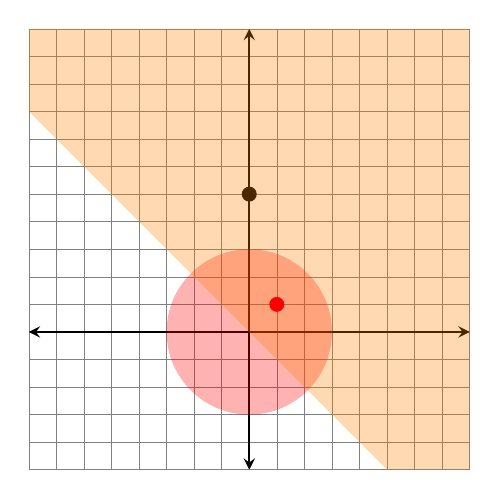
\begin{tikzpicture}[scale=0.35, >=stealth]
      \foreach \i in {\xMin,...,\xMax} {
          \draw [very thin,gray] (\i,\yMin) -- (\i,\yMax);
      }
      \foreach \i in {\yMin,...,\yMax} {
          \draw [very thin,gray] (\xMin,\i) -- (\xMax,\i);
      }
      \draw[<->, thick] (\xMin, 0) -- (\xMax, 0);
      \draw[<->, thick] (0, \yMin) -- (0, \yMax);
      \fill[fill=red, fill opacity=0.3] (0, 0) circle [radius=3];
      \draw[fill=black] (0, 5) circle [radius=0.25];
      \fill[fill=orange, fill opacity=0.3]
      (\xMin, -\xMin) -- (\xMin, \yMax) -- (\xMax, \yMax) -- (\xMax, \yMin) --
      (-\yMin, \yMin) -- cycle;
      \draw[red,fill=red] (1, 1) circle [radius=0.25];
    \end{tikzpicture}
    \caption{The orange region is unsafe because it intersects the red circle.}
    \label{fig:robot-unsafe}
  \end{minipage}%
%  \dotfill
  \hfil
\end{figure}

\begin{figure}[t]
  \centering
\end{figure}

Reflecting on our two admittedly informal proofs so far,
  we can boil them each down into three essential proof steps:
  (1) identify a set of positions $I$ that
  (2) contains all reachable positions; and that
  (3) does not intersect the red circle.
Each proof step is important.
Proof step (1) requires some creativity and foresight
  to pick a set that will make proof steps (2) and (3) possible.
Proof step (3) has been fairly straightforward so far,
  because we can visually analyze our set and the red circle
  to determine if they overlap.
If we wanted to be more precise about proof step (3),
  we could do some algebra to show that
  any position $(x, y)$ that satisfies the linear inequalities
  that define the polygonal regions from
    \cref{fig:robot-reachable,fig:robot-inductive-invariant}
  always fall outside the red circle,
  i.e. $\sqrt{x^2 + y^2} > 3$.

Proof step (2) is more subtle.
We have claimed informally that the robot will never
  be able to move southwest of the line $x + y = 5$,
  nor west of the $y$ axis,
  but what would constitute a more detailed proof of this fact?
These claims are claims of \emph{invariance},
  i.e., that the set $I$ from proof step (1) is an invariant,
  where an invariant is a set that contains all reachable positions.
The key to proving invariance is an \emph{inductive} argument,
  which first shows (2.1) that the initial position is in $I$
  and then shows (2.2) that, from any position in $I$,
  all steps the robot could take
  lead to new positions that are also in $I$.
By induction, this implies that all reachable positions
  are contained in $I$.
For the invariants represented in
  \cref{fig:robot-reachable,fig:robot-inductive-invariant}
  we could make proof steps (2.1) and (2.2) more precise
  by showing that the initial position
    satisfies the linear inequalities for the polygonal regions
  and by showing that if $(x,y)$ satisfies the inequalities,
    then so do both $(x, y+1)$ (moving due north)
      and $(x+1, y-1)$ (moving southeast).

\begin{figure}[t]%
%  \centering%
  \hfil%
  \begin{minipage}{0.45\linewidth}
    \centering
      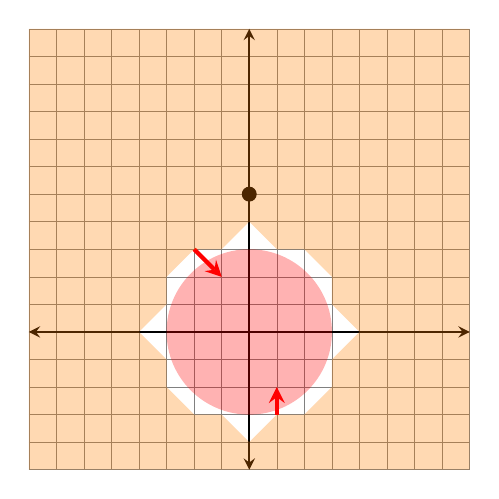
\begin{tikzpicture}[scale=0.35, >=stealth]
        \foreach \i in {\xMin,...,\xMax} {
            \draw [very thin,gray] (\i,\yMin) -- (\i,\yMax);
        }
        \foreach \i in {\yMin,...,\yMax} {
            \draw [very thin,gray] (\xMin,\i) -- (\xMax,\i);
        }
        \draw[<->, thick] (\xMin, 0) -- (\xMax, 0);
        \draw[<->, thick] (0, \yMin) -- (0, \yMax);
        \fill[fill=red, fill opacity=0.3] (0, 0) circle [radius=3];
        \draw[fill=black] (0, 5) circle [radius=0.25];
        \draw[red, ->, line width=1.5pt] (-2, 3) -- +(1, -1);
        \draw[red, ->, line width=1.5pt] (1, -3) -- +(0, 1);
        \fill[even odd rule, fill=orange, fill opacity=0.3]
        (0, 4) -- ++(1, -1) -- ++(1, 0) -- ++(1, -1) -- ++(0, -1) -- ++(1, -1)
               -- ++(-1, -1) -- ++(0, -1) -- ++(-1, -1) -- ++(-1, 0) -- ++(-1, -1)
               -- ++(-1, 1) -- ++(-1, 0) -- ++(-1, 1) -- ++(0, 1) -- ++(-1, 1)
               -- ++(1, 1) -- ++(0, 1) -- ++(1, 1) -- ++(1, 0) -- ++(1, 1)
               -- cycle
        (\xMin, \yMax) -- (\xMax, \yMax) -- (\xMax, \yMin) -- (\xMin, \yMin) -- cycle;
      \end{tikzpicture}
    \caption{The region outside the circle is invariant but not inductive.}
    \label{fig:robot-cti1}
  \end{minipage}%
  \hfil%
  \begin{minipage}{0.45\linewidth}
    \centering
    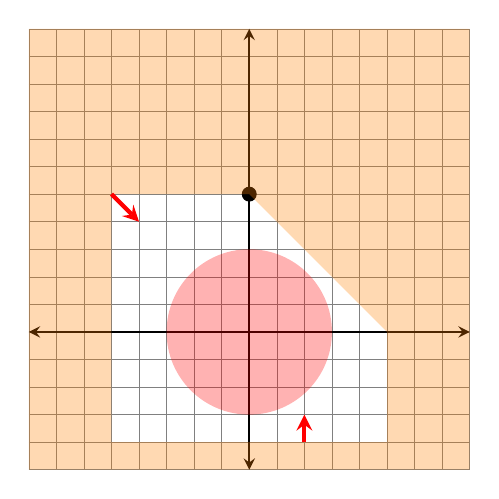
\begin{tikzpicture}[scale=0.35, >=stealth]
      \foreach \i in {\xMin,...,\xMax} {
          \draw [very thin,gray] (\i,\yMin) -- (\i,\yMax);
      }
      \foreach \i in {\yMin,...,\yMax} {
          \draw [very thin,gray] (\xMin,\i) -- (\xMax,\i);
      }
      \draw[<->, thick] (\xMin, 0) -- (\xMax, 0);
      \draw[<->, thick] (0, \yMin) -- (0, \yMax);
      \fill[fill=red, fill opacity=0.3] (0, 0) circle [radius=3];
      \draw[fill=black] (0, 5) circle [radius=0.25];
      \fill[even odd rule, fill=orange, fill opacity=0.3]
      (0, 5) -- (5, 0) -- (5, -4) -- (-5, -4) -- (-5, 5) -- cycle
      (\xMin, \yMax) -- (\xMax, \yMax) -- (\xMax, \yMin) -- (\xMin, \yMin) -- cycle;
      \draw[red, ->, line width=1.5pt] (-5, 5) -- (-4, 4);
      \draw[red, ->, line width=1.5pt] (2, -4) -- +(0, 1);
    \end{tikzpicture}
    \caption{This simplified region is also invariant but not inductive.}
    \label{fig:robot-cti2}
  \end{minipage}%
%  \dotfill
  \hfil
\end{figure}

It is instructive to see what happens when
  the set $I$ selected in proof step (1)
  fails due to proof steps (2) or (3).
When proof step (3) fails,
  $I$ intersects the red circle,
  as in \cref{fig:robot-unsafe}.
In this case we call the set $I$ ``unsafe''.
The small opaque red dot shows an example position that is both
  in the candidate set $I$ drawn as the orange region
  and the shaded red circle at the origin.
When proof step (2) fails,
  there is a position in $I$ from which
  the robot can step to a position outside $I$,
  as in \cref{fig:robot-cti1,fig:robot-cti2}.
The red arrows show examples of positions in the orange regions
  that can step out of orange regions.
We call such positions ``counterexamples to inductiveness'', or CTIs.

\begin{figure}[t]%
  \hfil%
  \begin{minipage}{0.45\linewidth}
    \centering
    \begin{tikzpicture}[scale=0.35, >=stealth]
      \foreach \i in {\xMin,...,\xMax} {
          \draw [very thin,gray] (\i,\yMin) -- (\i,\yMax);
      }
      \foreach \i in {\yMin,...,\yMax} {
          \draw [very thin,gray] (\xMin,\i) -- (\xMax,\i);
      }
      \draw[<->, thick] (\xMin, 0) -- (\xMax, 0);
      \draw[<->, thick] (0, \yMin) -- (0, \yMax);
      \fill[fill=red, fill opacity=0.3] (0, 0) circle [radius=3];
      \draw[fill=black] (0, 5) circle [radius=0.25];
      \fill[fill=violet, fill opacity=0.4] (0, 5) -- (3, 2) -- (3, 1) -- (4, 0) -- (4, \yMin) -- (\xMax, \yMin) -- (\xMax, \yMax) -- ($(-\yMax,\yMax)+(5,0)$) -- cycle;
    \end{tikzpicture}
    \caption{The largest safe inductive invariant for the robot.}
    \label{fig:robot-large-invariant}
  \end{minipage}%
  \hfil%
  \begin{minipage}{0.45\linewidth}
    \centering
    \begin{tikzpicture}[scale=0.35, >=stealth]
      \foreach \i in {\xMin,...,\xMax} {
          \draw [very thin,gray] (\i,\yMin) -- (\i,\yMax);
      }
      \foreach \i in {\yMin,...,\yMax} {
          \draw [very thin,gray] (\xMin,\i) -- (\xMax,\i);
      }
      \draw[<->, thick] (\xMin, 0) -- (\xMax, 0);
      \draw[<->, thick] (0, \yMin) -- (0, \yMax);
      \fill[fill=red, fill opacity=0.3] (0, 0) circle [radius=3];
      \draw[fill=black] (0, 5) circle [radius=0.25];
      \fill[fill=violet, fill opacity=0.4] (0, 5) -- (3, 2) -- (3, 1) -- (4, 0) -- (4, \yMin) -- (\xMax, \yMin) -- (\xMax, \yMax) -- ($(-\yMax,\yMax)+(5,0)$) -- cycle;
      \draw[->, red, line width=1.5pt] ($(-\yMax,\yMax)+(4,0)$) -- (2, 2);
      \draw[->, red, line width=1.5pt] (3, \yMin) -- (3, 0);
    \end{tikzpicture}
    \caption{Proof that every position outside the purple region is backward reachable.}
    \label{fig:robot-backward-reachable}
  \end{minipage}%
  \hfil
\end{figure}

In the robot example, we can rephrase inductiveness by saying:
  if a position $(x, y)$ is \emph{not} in $I$,
  then neither is any state due south or diagonally northwest of $(x, y)$.
Since our goal in any proof of the robot's safety is
  to come up with a set $I$ that is inductive and does not intersect the red circle,
  we know the states in the red circle must not be in $I$.
Using the rephrasing above,
  we can conclude that $I$ must also not contain
  any state due south or diagonally northwest of the red circle.
Continuing to rule out states in this way,
  we can find the \emph{largest} set $I$ that will make the proof go through,
  shown in \cref{fig:robot-large-invariant}.
To convince ourselves that this region $I$ is the largest safe inductive invariant,
  it is enough to show that every position not in $I$ is \emph{backward reachable},
  by which we mean, there is a sequence of steps
  starting from the position and ending somewhere in the red circle.
\Cref{fig:robot-backward-reachable} demonstrates that
  the positions just outside the purple region are all backward reachable,
  using sequences of steps that follow the red arrows to the red circle.
Every other position outside the purple shaded region
  is either due south or diagonally northwest of one of these two red arrows,
  and so is also backward reachable.

Because the robot example is so simple,
  we are able to exactly characterize
    the set of reachable states (\cref{fig:robot-reachable}) and
    the set of backward reachable states (\cref{fig:robot-backward-reachable}).
In more complex examples, this will be much more difficult,
  but luckily it will always be sufficient to find an overapproximation
  to the set of reachable states, such as \cref{fig:robot-inductive-invariant},
  which proves safety without exactly characterizing
  reachability or backward reachability.

\subsection{The robot example in set theory}

\def\robot{\ensuremath{\mathsf{robot}}}
\def\reach{\ensuremath{\mathsf{reach}}}

Let's formalize the robot example from the previous section
  using the language of set theory.

A \emph{transition system} $\tau = (S, S^0, \to)$ consists of a set of states $S$,
  a set of initial states $S^0\subseteq S$,
  and a binary transition relation $\to\subseteq S\times S$.
We write $s\to s'$ to mean $(s, s') \in \to$.

We can formalize the robot example as a transition system as follows.
\begin{align*}
  \tau_\robot &= (S_\robot, S^0_\robot, \to_\robot)\\
  S_\robot &= \set{(x,y) \mid x,y\in\Z}\\
  S^0_\robot &= \set{(0, 5)}\\
  \to_\robot &= \set{((x,y), (x, y + 1)) \mid x,y\in\Z} \mathrel{\cup}\\
            &\phantom{\mathrel{=}}\quad \set{((x,y), (x + 1, y - 1)) \mid x,y\in\Z}
\end{align*}

We write $s\to^* s'$ to mean that there is a (possibly empty) sequence of steps from $s$ to $s'$.
Using this notation, we can say that a state $s$ is \emph{reachable}
  if there is an initial state $s_0\in S^0$ such that $s_0 \to^* s$.
We write $\reach(\tau)$ for the set of reachable states of the transition system~$\tau$.

In the robot example,
  we characterized the set of reachable states in \cref{fig:robot-reachable}.
We can express the set precisely as
\[
  \reach(\tau_\robot) = \set{(x,y) \mid x \ge 0 \text{ and } x + y \ge 5}
\]
The proof of this fact follows the informal discussion from the previous section.
First, the set on the right hand side contains all reachable states,
  which can be shown with an inductive argument (which we spell out below).
Second, every state in this set is reachable,
  which we can show by
  first showing that everything on the diagonal $x + y = 5 \land x \ge 0$ is reachable
    (by a sequence of southeast moves from the initial state),
  and then showing that every state above the diagonal is reachable
    (by a subsequent sequence of north moves).

In the robot example, our goal was to prove the robot never falls in the red circle.
In general, the kinds of goals we will be interested in will be \emph{safety properties},
  specifically, that a transition system avoids a certain set of \emph{bad states} $B\subseteq S$
  that is claimed not to intersect the set of reachable states.
In the robot example, the bad states are the ones in the red circle:
\[
  B_\robot = \set{(x,y) \mid \sqrt{x^2 + y^2} \le 3}.
\]
The claim that the robot is \emph{safe} means that $B_\robot$ does not intersect $\reach(\tau_\robot)$,
  which is visually apparent in \cref{fig:robot-reachable}.

In simple systems, such as the robot example,
  $\reach(\tau)$ can be characterized directly,
  but in more complex systems, it is neither practical nor useful
  to obtain an exact characterization of reachable states.
Instead, one often uses \emph{overapproximations} to reachability,
  known as invariants.
We say that a set $I$ is an \emph{invariant} if it contains every reachable state,
  that is, if $\reach(\tau) \subseteq I$.
Thus, another way to talk about safety properties is to say that
  the complement of the set of bad states is an invariant,
  i.e. $\reach(\tau) \subseteq S\setminus B$.
Indeed, another way to set up the safety verification problem is
  to specify $S\setminus B$ directly instead of $B$,
  and to claim that $S\setminus B$ is an invariant.
We call this the \emph{positive phrasing of the safety problem}.

When $\reach(\tau)$ has a direct characterization,
  one can prove that $I$ is an invariant directly from the definition.
But in complex systems where
  no useful direct characterization of $\reach(\tau)$ exists,
  one instead uses an inductive argument to establish invariance.
We say that $I$ is an \emph{inductive invariant} if:
  (1) $S^0\subseteq I$; and
  (2) for any $s\in I$, if $s\to s'$, then $s' \in I$.

Both the green region from \cref{fig:robot-reachable} and
  the blue region from \cref{fig:robot-inductive-invariant}
  are invariants, and in fact are inductive invariants.
(Indeed $\reach(\tau)$ is always an inductive invariant in any transition system.)
However, not all invariants are inductive invariants.
For example, the orange regions from \cref{fig:robot-cti1,fig:robot-cti2}
  are both invariants (because they contain the green region from \cref{fig:robot-reachable})
  but neither are inductive.
If we wanted to use an inductive argument to show
  that these orange regions are invariants,
  we would need to first \emph{strengthen} them.

In general, suppose we want to prove that $I$ is an invariant of some transition system $\tau$,
  and that we don't have a useful direct characterization of $\reach(\tau)$ handy.
Further, suppose that $I$ is not inductive.
To show that $I$ is an invariant, it is enough to find another set $J$ such that:
  (1) $J\subseteq I$; and
  (2) $J$ is inductive.
Since $J$ is inductive, $J$ is an invariant, i.e. $\reach(\tau)\subseteq J$.
But $J\subseteq I$, so $I$ is also an invariant.
In the robot example, we could use the blue region from \cref{fig:robot-inductive-invariant}
  as an inductive strengthening
  to prove that either of the orange regions is an invariant.
Most of the art and skill of working with transition systems
  is in the ability to look at a non-inductive property
  and see what kinds of strengthenings of it
  might be good ideas to get it to be inductive.


\subsection{First-order logic for transition systems}\label{ssec:fol-tr}

We are on a journey to more and more formally specify the robot example
  and to prove its safety more and more automatically.
Our next stop is first-order logic,
  which we assume the reader is at least passingly familiar with.
(See \cref{sec:fol-background} for a formal presentation.)
The basic idea is to make the states of a transition system
  \emph{first-order structures} over \emph{state variables}, and
  to use formulas to describe the initial states,
  the transition relation, the bad states,
  and the inductive invariant.

For the robot, the state variables are $x$ and $y$,
  both of sort $\Z$.
A first order structure is just
  an assignment of variables to values of the correct sort.
In this case, a structure will be an integer for $x$ and an integer for $y$,
  that is, a pair of integers, or, in yet other words, a point in the plane.

The robot only has one initial state, $(5, 0)$.
We can describe this as a logical formula over the variables $x$ and $y$ as
\[
  \mathit{Init}_{\robot} ~~=~~ x = 0 \land y = 5.
\]

Taking the positive phrasing of the robot example's safety problem,
  we want to show that the set of states
  with distance strictly greater than 3 from the origin
  is an invariant of the transition system.
We can express this safety invariant as follows
  (avoiding square roots by squaring both sides)
\[
  \mathit{Safe}_{\robot} ~~=~~ x^2 + y^2 > 9.
\]

Since the initial condition and the safety condition
  of a transition system are \emph{sets} of states,
  they are encoded in logic as formulas over \emph{one} copy of the state variables.
The transition relation, on the other hand, is a \emph{binary relation},
  so it is encoded in logic as a formula over \emph{two} copies of the state variables.
(We refer to formulas over two copies of the state variables as
  "2-vocabulary" or "2-state" formulas,
  and we call the second copy of the variables "primed"
  and write them as $x'$, for example.)
In the robot example, we can write the transition relation as
\[
    \mathit{Tr}_{\robot} ~~=~~ (x' = x \land y' = y + 1) \lor (x' = x + 1 \land y' = y - 1).
\]
We think of the primed variables $x'$ and $y'$ as
  holding the values \emph{after} the step occurs,
while the unprimed versions hold the values from before the step.
The transition formula says:
\begin{quote}
  A step is possible from $(x, y)$ to $(x', y')$ if
    either $x$ stays the same and $y$ is incremented by one,
    or $x$ is incremented by one and $y$ is decremented by one.
\end{quote}

Next, we can state the blue region from \cref{fig:robot-inductive-invariant}
  as a formula
\[
  \mathit{Inv}_{\robot} ~~=~~ x + y \ge 5.
\]

If we are trying to prove $\mathit{Safe}$ using $\mathit{Inv}$,
  there are two things to check.
First, $\mathit{Inv}$ must be strong enough
  to prove $\mathit{Safe}$,
  that is,
\[
  \mathit{Inv} \Rightarrow \mathit{Safe}.
\]
In the robot example, this amounts to the fact that
  the blue region from \cref{fig:robot-inductive-invariant}
  does not intersect the red circle at the origin,
\[
  x + y \ge 5 \Rightarrow x^2 + y^2 > 9.
\]
Second, $\mathit{Inv}$ must be inductive,
  which is phrased logically using two formulas,
one to check that the initial condition implies the invariant,
\[
  \mathit{Init} \Rightarrow \mathit{Inv},
\]
and one to check that the invariant is preserved by the transition relation,
\[
  \mathit{Inv} \land \mathid{Tr} \Rightarrow \mathit{Inv}'.
\]
The first of these two formulas is over a single copy of the state.
But the second formula is a 2-vocabulary formula,
  both because it contains the 2-vocabulary formula $\mathid{Tr}$,
  and because we use $\mathit{Inv}'$ to mean ``$\mathit{Inv}$
  with all the state variables changed to their primed copy''.
In the robot example, there is only one initial state,
  so the check on initial states amounts the fact that
  the initial state is in the blue region
  or, logically,
\[
  x = 0 \land y = 5 \Rightarrow x + y \ge 5.
\]
To check that the blue region is preserved by the robot's steps,
  we need to observe that there is no way to start in a state in the blue region
  and take a step outside of it,
  or, logically,
\[
  x + y \ge 5 \land ((x' = x \land y' = y + 1) \lor
                     (x' = x + 1 \land y' = y - 1)) \Rightarrow
  x' + y' \ge 5.
\]
This formula is valid, since
  either $y' > y$ and $x' = x$ in the first kind of step,
  or $x + y = x' + y'$ in the second kind of step.
While a bit tedious, this is perhaps the first time in the robot example
  that we haven't had to hand-wave around
  the fact that one of the regions is inductive.
It follows from the tedium of checking this formula's validity.

\section{The Robot in \mypyvy}

It's finally time to write some \mypyvy.
Let's take a tour of the syntax using our robot example.
A \mypyvy program is a list of \emph{declarations}.
There are two broad kinds of declarations:
  those that define the transition system
  and those that make \emph{queries} over the transition system.

Here are two declarations for the state variables of the robot.%
\begin{lstlisting}[language=mypyvy, xleftmargin=.2\textwidth, xrightmargin=.2\textwidth]
mutable constant x: int
mutable constant y: int
\end{lstlisting}
In \mypyvy, we spell ``variable'' as ``\lstinline[language=mypyvy]{mutable constant}'',
  following the logical terminology of a constant symbol.
(We discuss mutability in more detail in the next section.)
All the state declarations together
  define the state space of the transition system.

The initial conditions are declared with the \lstinline[language=mypyvy]{init} keyword.
\begin{lstlisting}[language=mypyvy, xleftmargin=.2\textwidth, xrightmargin=.2\textwidth]
init x = 0
init y = 5
\end{lstlisting}
The conjunction of all the \lstinline[language=mypyvy]{init} declarations in a \mypyvy program
  is the initial condition of the resulting transition system.

The transition relation is declared
  with several \lstinline[language=mypyvy]{transition} declarations.
\begin{lstlisting}[language=mypyvy, xleftmargin=.2\textwidth, xrightmargin=.2\textwidth]
transition north()
  modifies y
  new(y) = y + 1

transition south_east()
  modifies x, y
  & new(x) = x + 1
  & new(y) = y - 1
\end{lstlisting}
Each \lstinline[language=mypyvy]{transition} has a name and takes parameters in parentheses,
  which are existentially quantified.
The \lstinline[language=mypyvy]{modifies} clause is a comma-separated list of state components
  that are changed by this transition;
  all other state components are implicitly constrained to not change.
For example, in the \lstinline[language=mypyvy]{north} transition,
  there is an implicit constraint $x' = x$,
  which was explicit when we were writing directly in first-order logic
  in the previous section.
In \mypyvy syntax, instead of primed symbols,
  we use the \lstinline[language=mypyvy]{new} keyword,
  so \lstinline[language=mypyvy]{new(y)} refers to $y'$.
\mypyvy also allows conjunction and disjunction symbols
  (\texttt{\&} and \texttt{|}) to appear \emph{before} the first conjunct or disjunct,
  for the sole reason that it makes it easy to vertically align
  the lines of a long formula.
The global transition relation of the transition system is
  the \emph{disjunction} of all the transition declarations in the program.

The safety property is declared using the \lstinline[language=mypyvy]{safety} keyword.
\begin{lstlisting}[language=mypyvy, xleftmargin=.2\textwidth, xrightmargin=.2\textwidth]
safety [no_fall_in] x * x + y * y > 9
\end{lstlisting}
A safety property can be given a name by including it in square brackets.
In this case the name is \texttt{no\_fall\_in}.
\mypyvy will use this name to refer to this invariant.
If no name is given, \mypyvy will refer to a line number instead.
If the program has more than one \lstinline[language=mypyvy]{safety} declaration,
  the safety property is the conjunction of all the declarations.
The \lstinline[language=mypyvy]{safety} keyword is our first example of
  a declaration that is a \emph{query}.
When processing the program, \mypyvy will attempt to prove that
  the safety property is true in all reachable states of the system.
As we have discussed throughout this chapter,
  the primary technique for proving a safety property is
  to find an inductive invariant.

These invariants are declared using the \lstinline[language=mypyvy]{invariant} keyword.
\begin{lstlisting}[language=mypyvy, xleftmargin=.2\textwidth, xrightmargin=.2\textwidth]
invariant x + y >= 5
\end{lstlisting}
Invariants can also be named, but here we choose to not name the invariant.
All the \lstinline[language=mypyvy]{invariant} declarations in a program are
  implicitly conjoined.

\begin{figure}[t]
%  \centering
  \begin{minipage}[b]{.4\textwidth}
  \begin{center}
  \begin{tabular}{c}
  \begin{lstlisting}[language=mypyvy, numbers=left]
  mutable constant x: int
  mutable constant y: int

  init x = 0
  init y = 5

  transition north()
    modifies y
    new(y) = y + 1

  transition south_east()
    modifies x, y
    & new(x) = x + 1
    & new(y) = y - 1

  # don't fall in!
  safety [no_fall_in]
    x * x + y * y > 9

  invariant x + y >= 5
  \end{lstlisting}
  \end{tabular}
  \end{center}
  \vspace{1.5cm}
  \caption{The complete robot example in \mypyvy.}
  \label{fig:robot-mypyvy}
  \end{minipage}%
  \hfil%
  \begin{minipage}[b]{.5\textwidth}
  \begin{center}
    {\footnotesize
  \begin{verbatim}
  checking init:
    implies invariant no_fall_in... ok.
    implies invariant on line 20... ok.
  checking transition north:
    preserves invariant no_fall_in... ok.
    preserves invariant on line 20... ok.
  checking transition south_east:
    preserves invariant no_fall_in... ok.
    preserves invariant on line 20... ok.
  all ok!
  ----------------------------------------
  checking init:
    implies invariant no_fall_in... ok.
  checking transition north:
    preserves invariant no_fall_in...
  state 0:
  x = 1
  y = -3
  state 1:
  x = 1
  y = -2
  error robot.pyv:17:1: invariant no_fall_in
      is not preserved by transition north
  error robot.pyv:7:1: this transition does
   not preserve invariant no_fall_in
  program has errors.
  \end{verbatim}
    }
  \end{center}
  \caption{\mypyvy output when running on two versions of the robot.}
  \label{fig:robot-mypyvy-output}
  \end{minipage}%
\end{figure}
That completes the robot example in \mypyvy.
Running \mypyvy on the resulting file causes it to
  issue queries to the solver to verify that the invariants
  are inductive and imply the safety property.
For this program, the verification succeeds.
\mypyvy's output can be seen in
  the top half of \cref{fig:robot-mypyvy-output}.
Commenting out the \lstinline[language=mypyvy]{invariant} declaration
  causes the verification to fail
  because the safety property is not itself inductive.
\mypyvy's output in this case can be seen in
  the bottom half of \cref{fig:robot-mypyvy-output}.
\mypyvy shows a counterexample to induction (CTI),
  which is a pair of states related by the transition relation
  (in this case, the \texttt{north} transition)
  such that the first state satisfies the candidate invariant
  but the second state does not.
The CTI in \cref{fig:robot-mypyvy-output} corresponds
  to the red arrow pointing north in \cref{fig:robot-cti1}.

\section{Background on first-order logic}\label{sec:fol-background}

In this section, we return to the basics of first-order logic.
The ideas of first-order logic are not complicated,
  but they are tedious to set up formally.
We will do our best.

\begin{figure}[t]
  \begin{gather*}
  \begin{array}{rcl}
    u &\in& \mathrm{String}\\
    s &::=& u \mid \mathsf{bool}\\
    t &\in& \mathrm{FunctionType}\\
    t &::=& (s,\dots,s) \to s\\
    \sigma &\in&  \mathrm{String} \rightharpoonup \mathrm{FunctionType}\\
    e &::=& \mathsf{true} \mid \mathsf{false} \mid \lnot e\mid e\land e\mid e\lor e \mid e \Rightarrow e \mid \\
      &   & e = e \mid f(e,\dots,e) \mid x \mid \forall x : s.\, e \mid \exists x : s.\, e
  \end{array}
  \end{gather*}
  \caption{Syntax of pure, multi-sorted first-order logic.}
  \label{fig:fol-syntax}
\end{figure}

%\todo{bummer that running example uses integers, which are not formalized in this section}

\Cref{fig:fol-syntax} describes the syntax of first-order logic.
A \emph{sort} $s$ is either $\mathsf{bool}$ or an uninterpreted symbol $u$.
A \emph{function type} $t$ is some number of argument sorts and a return sort.
A \emph{vocabulary} is a map from function names to function types.
We write $\mathsf{usorts}(\sigma)$ for the set of all uninterpreted sort
  symbols used in the type of any function symbol in $\sigma$.
We distinguish several special classes of function types.
If a function $c$ has zero arguments,
  then we say that $c$ is a \emph{constant},
  and in expressions we abbreviate $c()$ as $c$.
If a function $R$ has return type $\mathsf{bool}$,
  then we say that $R$ is a \emph{relation}.

An \emph{expression} is one of: a boolean constant,
  the application of a unary or binary boolean operation to subexpressions,
  an equation between expressions,
  the application of a function to some number of arguments,
  a variable,
  or a quantified expression.
There is a straightforward type system
  that assigns a sort (either an uninterpreted sort or $\mathsf{bool}$) to each expression,
  in the context of a vocabulary and a local context that binds variables to sorts.%
\footnote{Our approach to first-order logic is somewhat nonstandard,
in that we treat $\mathsf{bool}$ as ``just another sort'',
rather than having a separate syntactic category for formulas and terms.
This setup is somewhat more parsimonious in the presence of multiple uninterpreted sorts,
and it also has the advantage of allowing quantifying over booleans.
In any case, the fundamental expressivity of the logic is not changed by these choices.}
The type system also enforces that functions are applied to the correct number of arguments,
  that function arguments have types corresponding to the functions declared type in the vocabulary,
  and that both sides of an equation have the same type.
We omit the definition of this type system, and implicitly assume that all expressions are well typed.
We use the word \emph{formula} to mean ``an expression of type $\mathsf{bool}$''.

A \emph{first-order structure} $A$ over a vocabulary $\sigma$ is
 (1) a set $A_u$ for every uninterpreted sort $u\in\mathsf{usorts}(\sigma)$ and
 (2) for every function symbol $f\in\dom\sigma$
     with type $(s_1, \dots, s_n)\to s$,
     a corresponding mathematical function
     $A_f : A_{s_1} \times \dots \times A_{s_n} \to A_s$.
(In case one of the sorts is $\mathsf{bool}$, we define
  $A_{\mathsf{bool}} = \mathbb{B}$,
  \ie, every first-order structure interprets $\mathsf{bool}$
  as the set $\set{\top,\bot}$.)
We call $\bigcup_{u\in\mathsf{usorts}(\sigma)} A_u$ the \emph{universe} of $A$.

Given a vocabulary $\sigma$,
  a first-order structure $A$ over $\sigma$,
  an environment $\rho \in \mathrm{String} \rightharpoonup \bigcup_{u\in\mathsf{usorts}(\sigma)} A_u$,
  and a first-order expression $e$ of sort $s$,
  we define $\denote{e}_A^\rho$,
  the interpretation of $e$ in $A$, as follows.
\begin{gather*}
  \begin{array}{rcl}
  \denote{e}_A^\rho &\in& A_s\\
  \denote{\mathsf{true}}_A^\rho &=& \top\\
  \denote{\mathsf{false}}_A^\rho &=& \bot\\
  \denote{\lnot e}_A^\rho &=& \lnot \denote{e}_A^\rho\\
  \denote{e_1 \land e_2}_A^\rho &=& \denote{e_1}_A^\rho \land \denote{e_2}_A^\rho\\
  \denote{e_1 \lor e_2}_A^\rho &=& \denote{e_1}_A^\rho \lor \denote{e_2}_A^\rho\\
  \denote{e_1 \Rightarrow e_2}_A^\rho &=& \denote{e_1}_A^\rho \Rightarrow \denote{e_2}_A^\rho\\
  \denote{e_1 = e_2}_A^\rho &=& \denote{e_1}_A^\rho = \denote{e_2}_A^\rho\\
  \denote{f(e_1, \dots, e_n)}_A^\rho &=& A_f(\denote{e_1}_A^\rho, \dots, \denote{e_n}_A^\rho)  \\
  \denote{x}_A^\rho &=& \rho(x) \\
  \denote{\forall x : s.\, e}_A^\rho &=& \forall a\in A_s.\, \denote{e}_A^{\rho[x\mapsto a]}\\
  \denote{\exists x : s.\, e}_A^\rho &=& \exists a\in A_s.\, \denote{e}_A^{\rho[x\mapsto a]}\\
  \end{array}
\end{gather*}

If $e : \mathsf{bool}$ and $\denote{e}_A^\rho = \top$,
  then we say that $A$ is a \emph{model} of $e$,
  and we write $A \models e$.
We say that $e$ is \emph{satisfiable} if there exists a first order structure $A$ over $\sigma$ such that $A\models e$.
We say that $e$ is \emph{valid} if for every first order structure $A$ over $\sigma$, $A\models e$.
A formula $e$ is valid if and only if $\neg e$ is unsatisfiable (\ie, not satisfiable).
%
% equiv
If $e_1 : \mathsf{bool}$ and $e_2 : \mathsf{bool}$ are two formulas over $\sigma$,
then $e_1$  is \emph{semantically equivalent} to $e_2$ if for every structure $A$,
$A\models e_1$ if and only if $A\models e_2$.

Let $A$ be a first order structure over $\sigma$,
and for each $u\in\mathsf{usorts}(\sigma)$ let $B_u\subseteq A_u$.
Then define $B_f = A_f|_{B_{s_1}\times\dots\times B_{s_{n}}}$,
for each $f \in \dom\sigma$ of type $(s_1, \dots, s_n)\to s$.
Then in order for $B$ to be a first order structure,
we need it to be ``closed'' under all function symbols, \ie,
\[
  B_f(B_{s_1}, \dots, B_{s_n}) \subseteq B_s.
\]
(In the case that $s = \mathsf{bool}$, there is nothing to show here,
because $B_{\mathsf{bool}} = \set{\top, \bot} = A_{\mathsf{bool}}$.)
We call $B$ the ``restriction of $A$ to the $B_u$''.
It is sometimes convenient to gloss over the distinction between the different sorts $u$
and to speak of ``the restriction of $A$ to the set $X$'', where $X \subseteq \bigcup A_u$.
We say that $B$ is a \emph{substructure} of $A$ if $B$ is the restriction of $A$ to $\bigcup B_u$.
(This really just amounts to saying that $B$ is a first-order structure over $\sigma$
whose sets are subsets of $A$
and whose interpretation of every function symbol agrees with $A$'s interpretation.)

Substructures agree on the interpretation of quantifier free expressions,
as shown by the following lemma.
\begin{lemma}\label{lem:qf-denote-substruct}
  Let $e_0$ be quantifier free (not necessarily of sort $\mathsf{bool}$),
  and let $A$ and $B$ be first-order structures over $\sigma$
  such that $B$ is a substructure of $A$.
  Also, let $\rho \in \mathrm{String} \rightharpoonup \bigcup_{s\in\mathsf{usorts}(\sigma)} B_s$.
  Then $\denote{e}_B^\rho = \denote{e}_A^\rho$.

  Intuitively, a quantifier-free formula can only ``see'' elements
    of the structures $A$ and $B$
    if they are in the image of the interpretation of some function symbol,
    or if they are in the environment $\rho$.
  Since substructures agree on all function interpretations,
    the interpretation of $e_0$ can't change as we pass to the substructure $B$.
\end{lemma}
\begin{proof}
  Induction on $e$ using the definition of $\denote{\cdot}$.
\end{proof}

A formula $e : \mathsf{bool}$ is \emph{quantifier free}
  if its syntax does not contain any uses of $\forall$ or $\exists$.
A formula $e : \mathsf{bool}$ is called \emph{universal}
  if it is equivalent to a formula of the form $\forall^* e_0$, where $e_0$ is quantifier free.
(Here we use $\forall^*$ to abbreviate some (possibly empty) sequence of $\forall$ quantifiers over unknown sorts.)

Universal formulas have a special relationship with substructures, as shown by the following lemma.
\begin{lemma}\label{lem:univ-model-substruct}
  Let $e$ be universal and suppose $A\models e$ and that $B$ is a substructure of $A$.
  Then $B\models e$.

  Intuitively, $e$ says something about ``all'' elements of $A$, and
  there are no elements of $B$ that are not also elements of $A$, so
  $e$ also says the same thing about ``all'' elements of $B$.
\end{lemma}
\begin{proof}
  Write $e = \forall y_1 : s_1,\dots y_n : s_n.\, e_0$, where $e_0$ is quantifier free.
  Since $A\models e$, we know that for all $a_1\in A_{s_1}, \dots, a_n\in A_{s_n}$,
  $\denote{e_0}_A^{[y_1\mapsto a_1, \dots, y_n\mapsto a_n]} = \top$
  Now let $b_1\in B_{s_1}, \dots, b_n\in B_{s_n}$ be arbitrary.
  We need to show that $\denote{e_0}_B^{[y_1\mapsto b_1, \dots, y_n\mapsto b_n]} = \top$.

  Since $B$ is a substructure of $A$, we also have $b\in A_s$,
  and so we have $\denote{e_0}_A^{[y_1\mapsto b_1, \dots, y_n\mapsto b_n]} = \top$.
  Then by \cref{lem:qf-denote-substruct}, the left-hand side is equal to
  $\denote{e_0}_B^{[y_1\mapsto b_1, \dots, y_n\mapsto b_n]}$, which completes the proof.
\end{proof}


%
% basic EPR
If a vocabulary $\sigma$ consists of only relations and constants,
  then we call it ``function free''.
If $\sigma$ is function free and $e : \mathsf{bool}$ over $\sigma$,
  then we say that $e$ is \emph{effectively propositional for satisfiability}
  if $e$ is equivalent to a formula of the form $\exists^*\forall^*\, e_0$,
  where $e_0$ is some quantifier-free formula.
Taking the negation, we also obtain \emph{effectively propositional formulas for validity},
  which have the form $\forall^*\exists^*\, e_0$.
The fragment of first-order logic consisting of only effectively propositional formulas
  is known as ``effectively propositional reasoning'' or EPR.
When it is clear from context whether we are talking about satisfiability or validity,
  we allow ourselves to use the abbreviation ``$e$ is in EPR'' to mean one of the two notions above.

The reasons for defining these classes of formulas is that there are
  decision procedures for satisfiability and validity.

\begin{lemma}[Small model property]\label{lem:epr-small-model-property}
  Let $\sigma$ be function free,
  and let $e : \mathsf{bool}$ over $\sigma$ be effectively propositional for satisfiability.
  Then there exists a natural number $n$ (depending on $\sigma$ and $e$) such that
  $e$ is satisfiable if and only if it has a model of size at most $n$.

  Intuitively, since $e$ is EPR, after removing existential quantifiers, we are left with a universal formula.
  So given a model of $e$ we can construct a substructure consisting of only the interpretations
  of the existential variables and the constants of $\sigma$. Since the remainder of the formula is universal,
  it also holds in this substructure.
  Finally, the size of the substructure is bounded
  by the number of constant symbols in $\sigma$ plus the number of existential variables of $e$.
\end{lemma}
\begin{proof}
  Since $e$ is in EPR, we can write $e = \exists x_1, \dots, x_m.\, \forall y_1, \dots, y_k.\, e_0$,
  where one or both of $m$ and $k$ might be zero, and $e_0$ is quantifier free.
  Let $l$ be the number of constant symbols in $\sigma$, say $c_1, \dots, c_l$,
  and set $n = m + l$. We need to show $e$ is satisfiable iff it has a model of size at most $n$.
  The backwards direction follows directly.

  In the forwards direction, suppose $A \models e$ for some (possibly infinite) first-order structure $A$.
  Then peeling apart the interpretation of $e$ in $A$, we find that there must exist elements $a_1, \dots, a_m$
  of $A$ such that interpreting the $x_i$ as $a_i$ causes $e$ to come out true, \ie,
  \[
    \denote{\forall y_1, \dots, y_k.\, e_0}_A^{[x_1\mapsto a_1, \dots, x_m \mapsto a_m]} = \top.
  \]

  Now let $B$ be the restriction of $A$ to the set $X = \set{a_1, \dots, a_m, A_{c_1}, \dots, A_{c_l}}$.
  We claim $B$ is a model of $e$.
  First, we must show $B$ is closed under all function symbols.
  Since $\sigma$ is function free, we need only consider relations and constants.
  If $r\in\dom\sigma$ is a relation, then there is nothing to show,
  since we never restrict the interpretation of the boolean sort.
  If $c\in\dom\sigma$ is a constant, then $B_c() = A_c \in X$,
  since $X$ contains the interpretation of every constant symbol.

  By \cref{lem:univ-model-substruct},
  \[
    \denote{\forall y_1, \dots, y_k.\, e_0}_B^{[x_1\mapsto a_1, \dots, x_m \mapsto a_m]} = \top,
  \]
  and the result follows.
\end{proof}

Decidability of EPR follows as a corollary, after the following lemma.
\begin{lemma}\label{lem:finitely-many-structures}
  Given a fixed (finite!) vocabulary $\sigma$ (not necessarily function free),
  there are only finitely many first-order structures of any particular universe size.
\end{lemma}
\begin{proof}
  Fix a particular universe size $n$. Then for each constant symbol $c$ in
  $\sigma$, there are at most $n$ choices of how to interpret $c$ in the universe.
  For each relation symbol $R$, there are at most $2^{nk}$ choices for how to interpret $R$, where $k$ is the arity of $R$.
  And for each function symbol $f$, there are at most $n^{nk}$, where $k$ is there arity of $f$.
  Taking the product of all these choices across all symbols in $\sigma$ gives us an upper bound on the number of first order structures
  over $\sigma$ with universe size $n$.
\end{proof}

\begin{theorem}
  Let $\sigma$ be function free,
  and let $e : \mathsf{bool}$ over $\sigma$ be effectively propositional for satisfiability.
  Then it is decidable whether $e$ is satisfiable.
\end{theorem}
\begin{proof}
  By \cref{lem:epr-small-model-property}, it suffices to check for a model of up to size $n$,
  where $n$ is the number of constants in $\sigma$
  plus the number of existentially quantified variables of $e$.
  Then by \cref{lem:finitely-many-structures},
  there are finitely many structures of size at most $n$.
  We can enumerate them and check for each one
  whether it is a model of $e$.
  If we find a model, $e$ is satisfiable.
  If we exhaust all structures of size at most $n$,
  then we know no model of $e$ exists of any size (even infinite!).
\end{proof}

% stratified functions


\section{Expressing Transition Systems in \mypyvy}\label{sec:mypyvy-expressing-ts}

\mypyvy consists of a language for expressing transition systems (this section)
  and a tool for answering queries about such systems (\cref{sec:mypyvy-queries}).
The \mypyvy language closely corresponds to
  the theoretical development of first-order logic from \cref{sec:fol-background}.

A \mypyvy file consists of a sequence of declarations,
  which together define a transition system.
Recall that a transition system consists of a state space,
  a set of initial states,
  and a transition relation.
There are declarations for all of these things.
In addition, there are declarations to record other properties of interest,
  such as inductive invariants and safety properties.
While not officially part of the definition of the transition system,
  it makes sense to record these properties in the same file,
  so that queries about the system can make easy use of them.
For example, there is a query to check that all the invariants in a file
  actually are invariants.

% \todo{mypyvy should really not use the word \texttt{invariant} when we mean \emph{inductive}}

A transition system consists of a state space, a set of initial states, and a transition relation.
\mypyvy has one or more declarations corresponding to each of these components.

To define the state space,
  \mypyvy supports declaring uninterpreted sorts, constants, relations, and functions.
The \lstinline[language=mypyvy]{sort} keyword declares the name of an uninterpreted sort.
Uninterpreted sorts can be used in the types of other declarations in the file.
The state consists of constants, relations, and functions, which we refer to as ``state variables''.
Each state variable can by \lstinline[language=mypyvy]{immutable} or \lstinline[language=mypyvy]{mutable}.
An \lstinline[language=mypyvy]{immutable} state variable cannot be changed by the transition relation throughout an execution of the system,
  while a \lstinline[language=mypyvy]{mutable} state variable can evolve over time.
There are keywords \lstinline[language=mypyvy]{constant}, \lstinline[language=mypyvy]{relation}, and \lstinline[language=mypyvy]{function}
  for each category of state variable.
Here are some examples of sort declarations and state variable declarations.
\begin{lstlisting}[language=mypyvy, xleftmargin=.2\textwidth, xrightmargin=.2\textwidth]
  sort A
  immutable constant source: A
  mutable relation r(A)
  immutable function f(A): A
\end{lstlisting}
Each state variable declaration starts with its mutability, then its category, followed by its name.
After the name, the sorts of the arguments (if any) are given,
followed by a return type (if any; relations always return \lstinline[language=mypyvy]{bool}).

To define the initial conditions,
  \mypyvy provides the \lstinline[language=mypyvy]{init} keyword.
An \lstinline[language=mypyvy]{init} declaration consists of this keyword
  followed by a 1-state expression of type \lstinline[language=mypyvy]{bool}.
For example, the following declaration says that initially
  the relation \lstinline[language=mypyvy]{r} contains only the element \lstinline[language=mypyvy]{source}.
\begin{lstlisting}[language=mypyvy, xleftmargin=.2\textwidth, xrightmargin=.2\textwidth]
  init forall X:A. r(X) <-> X = source
\end{lstlisting}
If a file contains more than one \lstinline[language=mypyvy]{init} declaration,
  they are all conjoined together to form the initial condition for the transition system.

To define the transition relation,
  \mypyvy provides the \lstinline[language=mypyvy]{transition} keyword.
A \lstinline[language=mypyvy]{transition} declaration consists of this keyword
  followed by a name and some number of comma-separated parameters in parentheses,
  then a modifies clause,
  and then a 2-state expression of type \lstinline[language=mypyvy]{bool}.
For example, the following transition says that for any element
  currently in the \lstinline[language=mypyvy]{r} relation,
  you can add its image under the function \lstinline[language=mypyvy]{f}
  to \lstinline[language=mypyvy]{r} as well.
\begin{lstlisting}[language=mypyvy, xleftmargin=.2\textwidth, xrightmargin=.2\textwidth]
transition step(x: A)
  modifies r
  & r(x)
  & (forall X. new(r(X)) <-> r(X) | X = f(x))
\end{lstlisting}
The transition is named \lstinline[language=mypyvy]{step} and takes one parameter
  called \lstinline[language=mypyvy]{x} of type \lstinline[language=mypyvy]{A}.
Parameters are implicitly existentially quantified in the global transition relation.
The modifies clause declares which mutable state components are changed by the transition.
For any mutable state component \emph{not} in the modifies clause,
  \mypyvy implicitly adds a conjunct to the transition saying that
  that component does not change.
If there is more than one \lstinline[language=mypyvy]{transition} declaration in the file,
  then their \emph{disjunction} forms the transition relation of the transition system.

The \lstinline[language=mypyvy]{invariant} declaration takes a 1-state expression
  and conjoins it to the inductive invariant for the transition system.
\mypyvy can check that the resulting conjunction is actually an inductive invariant.
Some invariants can be marked with the The \lstinline[language=mypyvy]{safety} keyword instead,
  which indicates that these conjuncts are the ``specification'' of the transition system,
  and that the non-\lstinline[language=mypyvy]{safety} conjuncts are only there
  to make the invariant inductive.
For example, consider the following two \lstinline[language=mypyvy]{safety} declarations.
\begin{lstlisting}[language=mypyvy, xleftmargin=.2\textwidth, xrightmargin=.2\textwidth]
# oops! not true initially
safety forall X. r(X) -> exists Y. X = f(Y)

# true and inductive
safety forall X. r(X) -> X = source | exists Y. X = f(Y)
\end{lstlisting}
In the transition system example of this section,
  the first declaration says that every member of the relation \lstinline[language=mypyvy]{r}
  is in the image of the function \lstinline[language=mypyvy]{f}.
This is not true in the initial state, though,
  since \lstinline[language=mypyvy]{source} might not be in the image of \lstinline[language=mypyvy]{f}.
The second declaration fixes this problem by saying that
  every member of the relation \lstinline[language=mypyvy]{r}
  is either equal to \lstinline[language=mypyvy]{source}
  or is in the image of the function \lstinline[language=mypyvy]{f}.

The immutable symbols of a transition system form a sort of ``background theory'' for the system.
\mypyvy provides the \lstinline[language=mypyvy]{axiom} declaration,
  which takes a 0-state formula and adds it as an axiom of the background theory.
For example, we can use axioms to model the existence of a total order on a sort.
\begin{lstlisting}[language=mypyvy, xleftmargin=.2\textwidth, xrightmargin=.2\textwidth]
sort A
immutable relation le(A, A)
axiom le(X, X)
axiom le(X, Y) & le(Y, X) -> X = Y
axiom le(X, Y) & le(Y, Z) -> le(X, Z)
axiom le(X, Y) | le(Y, X)
\end{lstlisting}
Since the immutable relations are never updated by the transition relation,
  these axioms are true in every state.

The \lstinline[language=mypyvy]{theorem} declaration takes a $k$-state formula and
  ensures its validity given the background theory.
This can be used to prove that two alternate formulations of an invariant are equivalent,
  for example, or that one invariant or safety property implies another.
For example, given the background theory about \lstinline[language=mypyvy]{le} above,
  we could state a simple corollary that \lstinline[language=mypyvy]{le} is ``3-transitive''.
\begin{lstlisting}[language=mypyvy, xleftmargin=.2\textwidth, xrightmargin=.2\textwidth]
zerostate theorem
  le(X, Y) & le(Y, Z) & le(Z, W) -> le(X, W)
\end{lstlisting}
\mypyvy can check the validity of these theorems. See the next section.

\subsection{$k$-state expressions}

The expressions of \mypyvy closely follow those of first-order logic.
When reasoning about a transition system,
  one often has two copies of the state components in scope,
  those from the pre-state of a transition, and those from the post-state.
These two copies of the state components share a single copy of the immutable components;
  only the mutable components are duplicated.
An expression can refer to the post-state copy of a mutable symbol
  using the \lstinline[language=mypyvy]{new} operator,
  as in \lstinline[language=mypyvy]{new(r(X))}.
We call such expressions 2-state expressions.
For example, the body of each transition is a 2-state expression.
In contrast, many other expressions are
  more accurately referred to as 1-state expressions,
  meaning they only have one copy of the mutable symbols in scope.
For example, safety properties, invariants,
  and initial conditions all contain 1-state expressions.
Additionally, some expressions have \emph{no} copies of the mutable symbols in scope.
We call these 0-state expressions.
Axioms are the primary example of 0-state expressions;
  they can only refer to the immutable symbols.

In fact, further generalizations are possible
  to $k$-state expressions for any natural number $k$.
For example, one could write a 3-state expression,
  which describes a sequence of 3 states,
  where the first state's components are referred to directly,
  the second state's components use \lstinline[language=mypyvy]{new},
  and the third state's component use two applications of \lstinline[language=mypyvy]{new}.
Internally, \mypyvy fully supports $k$-state expressions,
  but their only user-facing appearance is in trace queries,
  which allow a customized form of bounded model checking.

A $k$-state formula can be thought of as a first-order formula
  over an extended vocabulary with $k$ copies of the mutable symbols.
A model for a $k$-state formula is a model for this first-order formula,
  \ie, a first-order structure that assigns interpretations to $k$ copies of the mutable symbols.
Models of $k$-state formulas often arise in the answers to queries over transition systems, 
  described in the next section.

\section{Queries on Transition Systems}\label{sec:mypyvy-queries}

\mypyvy supports several solver-aided queries over transition systems.

\paragraph{Inductiveness checking.}
The most common query is to check that
  the invariant specified in the file is an inductive invariant
  of the transition system.
\mypyvy performs this query on a file
  when run with the \texttt{mypyvy verify} subcommand.
As described at a high level in \cref{ssec:fol-tr},
  checking inductiveness consists of proving validity of the two formulas:
\[
  \mathit{Init} \Rightarrow \mathit{Inv},
\]
and
\[
  \mathit{Inv} \land \mathid{Tr} \Rightarrow \mathit{Inv}'.
\]
In the context of \mypyvy,
  $\mathit{Init}$ is the conjunction of all \lstinline[language=mypyvy]{init} declarations,
  $\mathit{Inv}$ is the conjunction of all \lstinline[language=mypyvy]{invariant} declarations, and
  $\mathit{Tr}$ is the \emph{disjunction} of all \lstinline[language=mypyvy]{transition} declarations.
Also, the prime symbol ($'$) is written \lstinline[language=mypyvy]{new(...)} in \mypyvy.
These two high-level queries can easily be directly expressed to the underlying solver.
As usual, to prove validity using a satisfiability solver,
  we negate the formula and hope for an \texttt{unsat} result.
In fact, \mypyvy performs one small optimization,
  which is to expand all top-level disjunctions outside the solver.
Instead of issuing a single query for the entire transition relation,
  \mypyvy issues separate queries for each transition.
Similarly, though perhaps less obviously,
  since the right-hand side of each query's implication is a conjunction,
  after the validity-to-satisfiability negation,
  this also becomes a disjunction at the solver level,
  and \mypyvy issues separate queries for each conjunct in the invariant.
So in total, if there are $n$ invariants and $m$ transitions,
  \mypyvy issues $n$ 1-state queries to check that the initial states satisfy the invariant,
  plus $mn$ 2-state queries to check that all invariants are preserved by all transitions.
In our anecdotal experience,
  splitting these disjunctions outside the solver improves performance and reliability,
  and, best of all, when something is taking a long time (usually because something is not inductive),
  the user can see what transition and invariant conjunct the solver is stuck on,
  improving transparency of the tool.

\paragraph{Bounded model checking.}
Given a transition system and a safety property,
  bounded model checking (BMC) asks,
  ``Is there a counterexample to safety in up to $k$ transitions?''
\mypyvy expresses this query to the underlying solver by ``unrolling,''
  that is, by making $k+1$ copies of the mutable state variables such that:
  (1) the first copy satisfies the initial conditions;
  (2) the last copy \emph{violates} safety;
  (3) all adjacent pairs of states are related by the transition relation.
If the solver finds a model for this query,
  it can be interpreted as an execution trace
  that starts in an initial states, and takes some sequence of transitions
  until it reaches a state that violates safety.
Such an example indicates a problem with
  either the transition system or the safety property.

The na\"{i}ve approach to bounded model checking described here does not scale
  as $k$ grows and as the transition relation becomes more and more disjunctive (\ie, more transitions).
Partially to workaround these scalability problems,
  \mypyvy also supports ``trace queries.''

\paragraph{Trace queries.}
A trace query is ``just'' a $k$-state formula,
  whose satisfiability encodes some kind of restricted reachability property
  that the user is interested in.
For example, in a model of a distributed system with many actions,
  na\"{i}ve BMC will only scale to a small depth, say 5 actions,
  in a reasonable amount of time,
  but many interesting behaviors of the system may not occur until a much greater depth,
  say 10 or 15 actions.
Of course, to gain confidence about all reachable states, no matter how deep,
  the user should prove an inductive invariant that implies safety.
But during testing, it can be convenient to explore deeper into the state space
  without needing to come up with an invariant.
The user can write a trace query which pares down the set of transitions
  to explore at each step.
For example, if the distributed system starts by electing a leader
  before accepting further requests,
  the user can create a trace query,
  which lists a sequence of transitions
  that result in a leader being elected,
  followed by a sequence of transitions to accept a request.
At the end of this sequence, the user can include an assertion,
  such as ``the final state reached on this trace violates safety.''
The resulting $k$-state expression can be checked for satisfiability.
If it is unsatisfiable, then there is no execution violating safety.
Trace queries can be solved at a much higher depth than BMC
  because each step of the execution is constrained to execute
  a single kind of transition (or just a handful of transitions),
  rather than the disjunction of all possible transitions.
This helps the solver not get confused
  enumerating many different possible combinations.

In addition to trace queries that are expected to be unsatisfiable,
  it is also useful to make trace queries that are expected to be satisfiable,
  to check, \eg, that there is at least one execution where a leader gets elected successfully.
This latter kind of query is especially useful for detecting vacuity bugs,
  where a typo in the formal model causes one or more transitions
  to be equivalent to \textsf{false}.
Vacuity bugs are impossible to detect by proving inductive invariants,
  because every invariant is preserved by \textsf{false}!
So trace queries become a crucial tool to ensure a transition system
  accurately reflects its author's understanding and intentions.

\paragraph{Theorems.}
\mypyvy's \lstinline[language=mypyvy]{theorem} declaration checks
  the validity of a $k$-state formula in the background theory of the transition system,
  as discussed in \cref{sec:mypyvy-expressing-ts}.
Although the syntax is quite different from trace queries,
  the implementation is very similar.
A trace query is a $k$-state formula that the user declares to be
  ``expected satisfiable'' or ``expected unsatisfiable''.
On the other hand, a theorem is $k$-state formula that the user
  declares is ``expected valid'', \ie, its negation is expected to be unsatisfiable.

Together, trace queries and the \lstinline[language=mypyvy]{theorem} declaration
  cover three out of the four possibilities
  of the satisfiable/unsatisfiable and negated/not-negated dimensions.
The remaining possibility would be a formula whose negation is expected to be satisfiable.
A reasonable name for this idea would be ``nonvacuous,''
  and it seems in principle that it could be as useful as satisfiable trace queries are.
A future version of \mypyvy may unify trace queries and theorems
  into one syntactic declaration form,
  and allow for ``nonvacuous'' queries as well.

\paragraph{Universal Property-Directed Reachability (\updr).}
\mypyvy includes an implementation of \updr,
  which can infer universally quantified inductive invariants
  in pure first-order logic (\ie, without arithmetic)~\cite{updr-jacm}.
\updr takes a transition system and a desired safety property
  and tries to construct an inductive invariant which implies safety.
If it succeeds, it returns the inductive invariant.
If it does not succeed,
  \updr can either loop forever or return a ``relaxed  counterexample''.
A relaxed counterexample \emph{proves} that
  there is no universally quantified inductive invariant that implies safety.
A relaxed counterexample consists of a sequence of interleaved
  transitions from the transition system and ``relaxation steps'',
  which are steps where some elements of some sorts get deleted.

The space of possible invariants inferred by \updr are
  conjunctions of universally quantified clauses of pure literals.
By pure literal, we mean either a pure atom or its negation,
  and by pure atom we mean either a relational fact over variables,
  an equation between a constant and a variable,
  or an equation between a function applied to variables and a variable.
The reason for this seemingly obscure search space is
  due to the way \updr constructs candidate invariants,
  which is by finding backwards reachable states and then ``blocking'' them
  by computing a ``forbidden sub-state'' that
  rules out all states with a certain pattern of relation/constant/function facts.
By default, when asked to perform \updr,
  \mypyvy uses the invariants in the file marked \lstinline[language=mypyvy]{safety}
  as the target property.
\mypyvy's implementation of \updr has been a useful baseline
  for other invariant inference research to compare against,
  see, \eg, Phase-\updr~\cite{phase-updr}.

\paragraph{Answers to queries, or, how to read counterexamples.}
While each of the above queries is quite different,
  they all occasionally return answers
  that involve models of $k$-state formulas.
For example, when inductiveness checking fails,
  it returns either
    a $1$-state model demonstrating a violation of safety in an initial state,
    or a $2$-state model demonstrating a counterexample to induction.
As another example,
  when bounded model checking finds an execution that violates safety,
    it returns a $k$-state model witnessing the executions trace.
Queries often have other possible outputs besides $k$-state models,
  \eg, ``verified'' or ``no trace found'' or,
  for \updr, a formula that is an inductive invariant proving safety.
But these other outputs are either simple
  or have well understood existing output formats.

We have already seen one example
  of \mypyvy's output format for displaying $k$-state models:
  the bottom half of \cref{fig:robot-mypyvy-output}
  shows a CTI (\ie, a 2-state model) for the robot system.
In that example, the 2-state model is printed
  by showing the values of all the variables
  in state 0 and in state 1.
More generally, for a model with $k$ states,
  \mypyvy first displays the values of all the \emph{immutable} symbols,
  and then, for each state, the values of the mutable symbols in that state.
For relational symbols,
  by default \mypyvy only prints positive literals,
  \ie, the tuples that are in the relation.

\paragraph{Annotations, plugins, and custom printers for states.}

\mypyvy answers queries by calling Z3,
  and \mypyvy prints whatever model Z3 returns, translated into \mypyvy syntax.
Often, solver models are strange and hard to read.
For example, if a transition system uses a total order relation on one of its sorts,
  it would make sense to always print that with names that are ordered by the total order,
  but Z3 is unlikely to do this by chance.
To improve the readability of the model format,
  \mypyvy supports custom formatting via printer plugins.

Every declaration in \mypyvy can be tagged with \emph{annotations},
  which have no inherent meaning,
  but can be detected by plugins to cause things to be printed differently.
Annotations come after the declaration they are attached to,
  are written with an at-sign (\lstinline[language=mypyvy]{@}),
  and can take arguments in parentheses, as in the following example.
\begin{lstlisting}[language=mypyvy, xleftmargin=.2\textwidth, xrightmargin=.2\textwidth]
  sort node @printed_by(ordered_by_printer, le)
\end{lstlisting}
This annotation tells \mypyvy that the sort \lstinline[language=mypyvy]{node}
  should be printed in the order given by the total order \lstinline[language=mypyvy]{le}.
The annotation name \lstinline[language=mypyvy]{printed_by}
  is detected by \mypyvy's model printing logic,
  and when such an annotation is found,
  it calls a plugin named by the first argument in the annotation,
  in this case \lstinline[language=mypyvy]{ordered_by_printer}.
That plugin uses the second expression as a relation name
  to look up the total order in the model,
  which is then used to order the elements of sort \lstinline[language=mypyvy]{node}
  before printing them.

\mypyvy supports several other custom printers,
  including one for printing sorts
  that represent sets of elements coming from another sort.
Users can also define their own printers by defining a printing plugin.
\mypyvy's proof of the Raft protocol comes with a custom printer
  for displaying Raft's logs in a readable way.

\mypyvy also supports a handful of other annotations.
\lstinline[language=mypyvy]{@no_print} instructs \mypyvy
  not to print a sort, relation, constant, or function at all,
  which can be useful either
  because a custom printer for another symbol also handles printing this symbol, or
  temporarily because the model is large and the symbol is irrelevant to the current debugging session.
\lstinline[language=mypyvy]{@no_minimize} is used
  to instruct \mypyvy's model minimizer not to minimize elements of a certain sort or relation.

The annotation framework is extensible, and we expect other uses of annotations will come up in the future.
We would like to thank Daniel Ricketts for his contributions to this aspect of \mypyvy.

% \section{Internals of \mypyvy}
%
% \begin{verbatim}
% - a tour of main()
% - the mental model of k-state formulas (correctly handling immutable)
%   - evaluating a k-state formula on a trace
% - philosophy on interacting with z3, the Solver class
% - how to write a mypyvy "plugin"
% - syntax.the_program and its consequences
% \end{verbatim}

\section{Using \mypyvy}

We have used \mypyvy as a platform to support several research projects
  in the general area of automated verification and invariant inference.

\paragraph{Another proof of Raft.}
In \cref{sec:verdi:casestudy-raft}, we discussed a Coq proof of
  the safety of Raft consensus protocol.
That effort involved over 50000 lines of proof for about 500 lines of code.
Using the automation of \mypyvy,
  and based on ideas from our collaborators on
  how to encode the proofs of Paxos and MultiPaxos/Raft in first-order logic~\cite{Padon-al:OOPSLA17, pldi18-mfd},
  we were able to produce another proof of Raft's safety in \mypyvy.
The \mypyvy proof is under 500 lines total,
  including both the model of the protocol and its invariants.%
\footnote{\url{https://github.com/wilcoxjay/mypyvy/blob/5b5cb9f3be8a990ed14837638d541f5eebdfe88f/examples/raft.pyv}}
The primary difficulty that remains in the proof is
  just to \emph{state} the inductive invariant that implies safety.
We hope to continue to improve the state of the art here
  through work on invariant inference,
  which would allow the proof to get even shorter and easier.

There are some important differences and tradeoffs between
  the Coq proof of Raft from \cref{chap:verdi}
  and the \mypyvy proof presented here.
First, the Coq proof yielded an executable implementation of the protocol
  via extraction to OCaml, which we were able to run and benchmark.
In contrast, the \mypyvy proof is merely about a logical model of the system.
Neither is clearly a better approach in all circumstances,
  given the massive effort-guarantee tradeoff present.
Second, the Coq proof is more \emph{foundational},
  meaning that any needed theory is developed from first principles.
For example, we developed a theory of linearizability and
  used it to prove Raft linearizable.
In contrast, the \mypyvy proof \emph{bakes in} many assumptions about linearizability, induction, and safety proofs.
Finally, the specifications are somewhat different.
The Coq proof proves linearizability,
  which is a property of the set of traces that make up the behaviors of the system.
In contrast, \mypyvy ``only'' proves what the Raft paper calls ``State Machine Safety''.
This safety property is still a deep result about the protocol,
  but it is somewhat simpler than the trace reasoning required to prove linearizability.
Overall, the proofs make different tradeoffs in the effort-results space,
  and we believe both are valuable.
Speaking anecdotally, we learned much from both efforts.
The fact that the Coq proof yielded an implementation meant
  that we were forced to consider practical concerns of efficiency, ensuring we didn't cut too many corners.
On the other hand, the \mypyvy proof gave us higher-level insight into ``why'' the protocol works,
  because the edit-verify-debug cycle was so much tighter, we were able to optimize our proof and really understand its guts.

\paragraph{Phase Invariants.}
Several projects have used \mypyvy's implementation of \updr as a baseline
  which can be extended and compared against in the hopes of improving invariant inference.
In one such project, we extended \updr with the idea of a \emph{phase automaton},
  a finite state machine whose states are labeled with invariants and
  whose edges are synchronized with transitions of the underlying transition system~\cite{phase-updr}.
Such an automaton captures the ``phase structure'' of the protocol,
  \eg, first elect a leader, then commit some log entries.
A labeled phase automaton is \emph{inductive} if, roughly speaking,
  the transitions on all edges in the automaton preserve the invariants on their incident nodes.
An \emph{unlabeled} or partially (noninductively) phase automaton
  poses a generalization of the invariant inference problem,
  where the goal is to infer a strengthening of the labels to make the automaton inductive.
This label inference problem can be solved by a generalization of \updr
  that simultaneously solves for the invariants of each node,
  passing proof obligations between them.
By providing a partial phase automaton,
  the user can help make the invariant inference problem easier,
  thus improving performance.

\paragraph{First-order Quantified Separators.}
Another project which uses \mypyvy as a platform
  to build improved invariant inference techniques,
  but which the author was not directly involved in,
  is \citeauthor{folic3}'s FOL-IC3 algorithm~\cite{folic3}.
\updr extends the propositional IC3/PDR algorithms to work on universal formulas.
Similarly, FOL-IC3 extends the same propositional algorithms to work on arbitrary quantified formulas.
The key insight of this work is to reduce the invariant inference problem to a \emph{separation} problem,
  which asks for a (quantified) first-order formula that can distinguish two given sets of example structures.

In addition to the three projects mentioned above,
  we have several ongoing pieces of work that use \mypyvy as a platform.
So far, it seems to be working out well!

\section{Related Work}

% \todo{introduce the expressiveness-automation spectrum, and place everybody on it}

\mypyvy is directly inspired by \ivy~\cite{Padon-al:PLDI16}.\footnote{
  \ivy's code is available on Github at \url{https://github.com/kenmcmil/ivy}.
  %
  See also the \ivy website at \url{http://microsoft.github.io/ivy/}.
}
%
The \ivy tool supports specification, implementation, and verification of systems,
including distributed and concurrent systems.
%
Systems are expressed as a set of \emph{actions},
each written in a simple imperative programming language
over state variables from a first-order vocabulary.
%
The verification queries \ivy asks of the underlying solver
are carefully designed to land in a decidable fragment of logic,
increasing the efficiency, reliability, and predictability
of the verification.
%
When verification fails, concrete counterexample traces
are shown to the user demonstrating the violation.
%
\ivy{} also has a powerful module system
that supports so-called ``circular'' assume-guarantee reasoning,
where all modules get to assume all other modules' invariants,
but are under the obligation to show that they do not violate
their own invariants.
%
(This reasoning is not actually circular, but sound,
because ``nobody violates their invariants first''
implies ``nobody violates their invariants''.)

One can view \mypyvy as similar to a hypothetical intermediate language
in \ivy{}'s pipeline to the solver.
%
\ivy{} compiles the modular imperative program
into a set of purely logical transition systems,
each of which must be verified.
%
One could imagine making this connection explicit,
by using \mypyvy as a ``backend'' for \ivy,
translating the transition systems into \mypyvy syntax.
%
This would have the advantage of making
\mypyvy's invariant inference algorithms available
to \ivy programs.
%
Indeed, many of the examples and benchmarks used by \mypyvy
were manually translated from \ivy.
%
We have begun work on such a translator,
and hope to continue to work more closely with \ivy in the future.


Dafny is a programming language
designed from the ground up for verification~\cite{Leino:LPAR10}.
%
Dafny is built on top of the Boogie intermediate verification language~\cite{boogie-manual},
which itself uses the Z3 SMT solver~\cite{z3}.
%
Dafny has an imperative object-oriented programming language with
objects, statements, loops, arrays, and heap-allocated data structures,
and has a rich Hoare logic for reasoning about these programs.
%
It also has a purely functional expression-oriented programming language
with first-class and higher-order functions, recursion, lists and logical quantifiers.
%
These logical features can be used express the specification of the imperative code,
or they can be used by themselves, turning Dafny into more of a proof assistant
than a programming language.
%
Dafny enjoys a high degree of proof automation, since all obligations are
eventually sent to Z3.
%
However, these queries can have complex quantifier structure to them, meaning
that they typically do not fall into any decidable fragment of first-order logic.
%
Dafny instructs Z3 to use syntactic heuristics based on E-matching
to manage quantifier instantiation process~\cite{z3-e-matching,simplify}.
%
This approach achieves good performance in practice,
but it means that the solver cannot return counterexamples,
and that the user must have a basic understanding of E-matching
in order to be an expert user of quantifiers in Dafny.

Previous chapters of this thesis used the \Coq proof assistant~\cite{Coq}.
%
\Coq is an interactive theorem prover and purely functional programming language
based on dependent type theory.
%
Its design gives it essentially limitless expressiveness,
but this comes at the cost of manual proof effort.
%
\Coq is the perfect tool for the job of building a new logic,
like we did in \cref{chap:disel} with \disel.
%
Also, \Coq has support for building domain-specific proof automation,
as promoted by \citet{chlipala:cpdt},
so with careful design, one can greatly reduce manual proof effort.
%
\mypyvy places itself at a very different point in the design space,
constraining what the programmer can write to a first-order transition system,
and in return, giving essentially full automation.
%
%\todo{move the rest of this somewhere reasonable}
%
My own journey as a researcher has taken me through many points
on this spectrum.
%
I have seen the benefits of being able to transliterate
your mathematical theorem statements directly into a Coq proposition,
but I have also seen the beauty of not having to write any proofs.
%
In any particular domain, it often makes sense for the community to
begin by building tools in very expressive frameworks,
because we don't yet know what we will need.
%
After this initial step, researchers can start the process of
figuring out exactly what needs to be expressed,
and what can be traded away in exchange for better automation.

\TLA is a specification language for modeling systems
developed by \citet{lamport:tla,lamport:specifying-systems}.
%
It comes with a suite of tools to analyze models,
including tools for model checking and deductive theorem proving.
%
\citeauthor{lamport:tla} advocates for a style of using \TLA
where most of the benefit of the process is gained
just from formally expressing the model of the system,
because the user is forced to carefully think through the details.
%
Users can derive additional benefit by model checking their systems,
using the TLC bounded model checker~\cite{tlc}.
%
TLC is an explicit-state model checker that exhaustively explores
a finite version of the system (\eg, all Raft executions where
there at most 5 nodes, at most 2 commands, and at most 3 terms, etc.).
%
Users can go even further by using the \TLA proof system (TLAPS)
to prove their systems correct~\cite{tlaps}.
%
TLAPS uses a hierarchical (treelike) proof structure,
where the leaves of the tree can be dispatched by automated solvers.
%
The most interesting point of comparison for \mypyvy is
\TLA's language for specifying systems.
%
\TLA is much more expressive than \mypyvy,
allowing users to write arbitrary temporal logic formulas
to describe their system.
%
While sometimes needed, this expressiveness makes
analysis and proof more challenging,
and users often stay within an idiomatic subset that
constructs a transition relation as the finite disjunction of
parameterized actions.
%
One way to view \mypyvy is as a codification of this idiom into a language.
%
By restricting the way users write their system specifications,
\mypyvy is able to completely automatically analyze
the safety problem for these systems.
%
On the other hand, \mypyvy does not currently support liveness reasoning,
so users of \TLA would miss having access to that kind of reasoning.
%
We plan to investigate liveness in future work,
encoding the queries in first-order logic
following the approach of \citet{padon:reducing-liveness}.

nuSMV and nuXmv are symbolic model checkers,
originally based on BDDs and SAT solvers,
and later adopted to infinite-domain systems
by using SMT solvers~\cite{nusmv,nusmv2,nuxmv}.
%
These tools are ``workbenches'' that implement many different techniques
to attack the model checking problem.
%
This is similar in spirit to \mypyvy's goal of
providing a framework to implement several approaches.
%
One key difference between nuXmv and mypyvy is that
nuXmv's support for infinite-state systems
is based on integer and real number types,
while \mypyvy's primary way to reason about such systems
is based on pure first-order uninterpreted sorts.
%
In our experience, most distributed systems do not need
specific interpreted operations over numbers,
and instead are naturally expressed over uninterpreted sorts
using axioms for, e.g. a total order.

Historically, many model checkers intended for hardware have worked on the bit level,
\ie, treating each bit as a separate boolean variable.
%
This encoding allows the use of off-the-shelf SAT solvers,
but loses mujch of the high-level structure present in the original problem.
%
Recently, the community has developed several \emph{word-level} techniques,
that maintain this high-level information during solving.
%
AVR is one such word-level symbolic model checker
that has shown promise in the hardware model checking community~\cite{goel-avr}.
%
At its core, AVR uses syntax-guided abstraction to compute a
word-level model of the system in first-order logic,
which can then be analyzed with an implementation of IC3 on top of several SMT backend solvers
to infer an inductive invariant~\cite{bradley-ic3}.
%
Most closely related to \mypyvy is the subsequent tool I4~\cite{i4},
which builds on top of AVR's ability to efficiently verify finite-domain systems
to analyze infinite-state systems such as distributed protocols.
%
I4 works by constructing finite instances of the protocol,
analyzing them with AVR to get an inductive invariant for the finite protocol,
and then generalizing this invariant
to get a candidate invariant for the original protocol.
%
This candidate must then be verified using unbounded techniques,
such as \ivy~\cite{Padon-al:PLDI16},
and if a counterexample is obtained,
a larger finite instance of the protocol must be analyzed.
%
I4 reads protocols written in the \ivy input language.

Verification modulo theories (VMT)~\cite{nuxmv-user-manual,vmt-website}
is an extension of the SMT-LIB standard~\cite{smtlib-standard}
to support reasoning about symbolic transition systems.
%
Transition systems are defined by annotating a standard SMT-LIB function definition
with a special keyword marking it as the definition of the
initial conditions or transition relation.
%
Since transition relations are 2-state formulas,
as discussed in \cref{sec:mypyvy-expressing-ts},
VMT again uses special keywords to declare that a SMT-LIB variable is
the ``next'' variable corresponding to another variable.
%
Both safety properties (of the form $\Box\varphi$) and
liveness properties (of the form $\Diamond\Box\varphi$)
can also be specified in the VMT description of the transition system,
but other queries (such as bounded reachability queries or
\mypyvy-style ``trace'' queries) cannot be specified.

\mypyvy's $k$-state semantics for formulas is
related to interpretations of Linear Temporal Logic (LTL)
over finite traces~\cite{vardi-ltl-finite}.
%
A key difference in the \mypyvy setting is that
each state is a first-order structure,
rather than a propositional truth assignment.
%
It would be interesting to extend \mypyvy
with explicit temporal operators that are ``unrolled''
when translating to the solver.

Btor2 is a language for specifying word-level hardware model checking problems
over bitvectors and arrays~\cite{btor2}.
%
It is an extension of the well-known bit-level format AIGER~\cite{aiger-1.9},
which is used in the hardware model checking competition~\cite{hwmcc20}.
%
Both AIGER and Btor2 are tailored to the case of reasoning
about finite-state systems, especially those derived from hardware designs.
%
Thus, neither supports infinite or unbounded sorts,
which is the focus of \mypyvy.

\section{Conclusion}

In this chapter, we described \mypyvy, a language and tool
  for analyzing symbolic transition systems expressed in first-order logic.
\mypyvy has already outgrown its original purpose
  and has had a surprisingly successful beginning to its life.
There are several directions for future work, both internally facing and external.

\paragraph{Future Work.}

On the internals side, there are conceptual design choices
  that should be revisited in the interests of cleanliness.
For example, \mypyvy currently separately represents constants, relations, and functions
  as distinct kinds of objects,
  but it would be cleaner to represent everything as a function.
A similar kind of conceptual simplification seems possible with queries,
  since essentially every query (except for invariant inference queries)
  can be phrased as asking a satisfiability question about a $k$-state formula.
It would be nice to capture this insight into a more general query language
  that unifies inductiveness checking, background theory theorem proving,
  bounded model checking, and trace queries.
Another minor internal nit is that \mypyvy currently assumes
  that there is one global transition system under analysis.
This assumption makes sense in the context of a command line tool
  that is asked a simple query about a single file.
But in more sophisticated cases, the assumption breaks down.
For example, any kind of program transformation of the transition system itself
  causes there to be two transition systems in scope,
  which is currently difficult to work with, and we end up hacking around it.
It would be nice to remove this limitation.

Another aspect of \mypyvy's design worth revisiting is its interface to the underlying SMT solver.
\mypyvy was originally designed to use Z3's Python API,
  which was initially convenient and allowed rapid prototyping,
  but this has the downside that we cannot easily use other SMT solvers.
We have actually hacked in support for CVC4,
  but the mechanism for doing so it very unsavory:
  we use the Z3 API to build the query and then ask Z3 to print it in SMT-LIB format,
  which we then ship to CVC4.
A better solution would be to introduce some kind of mid-level solver interface,
  probably based on SMT-LIB,
  which would allow us to use multiple solvers easily.
An important design constraint here is that
  we don't want to give up the performance benefits
  of using the API for expensive queries such as \updr,
  which builds many ASTs with sharing efficiently using the API.


On the external side, there are endless possibilities for tools to build using \mypyvy.
For example, we have several ongoing projects related to invariant inference and improving \updr.
More generally, we are interested in building an ``IDE for transition systems,''
  which is able to give real-time feedback on the model as the user develops it.
Relatedly, we'd like to make invariant inference more interactive.
Currently, the execution model of \updr is a batch processing job,
  and a rather expensive one at that.
When \updr fails to find an invariant, it often seems to loop forever,
  giving no intermediate results or feedback to the user.
Instead, it would be nice to have an approach that
  could be stopped midway through inference
  and have its state inspected by the user,
  who could then guide the search.

Besides our own interests, there are also many other possible tools to build on top of \mypyvy.
We encourage readers to join us in the quest for user-friendly symbolic reasoning about transitions
  that is fast and works on interesting and practical examples.
These are hard problems, and there is much work to do. We need your help!
